\section{Pretrained Models Quickly Learn New Tasks}

After demonstrating that LIMA is competent in a variety of question-answering and text generation tasks, we now test the boundaries of what can be achieved with only 1,000 examples.
We challenge LIMA in both multi-turn dialogue and text generation with structural constraints, and discover that LIMA exhibits surprising levels of robustness to these new tasks, and that even a handful of related training examples can dramatically boost its capabilities.


\subsection{Multi-Turn Dialogue}

Can a model fine-tuned on only 1,000 single-turn interactions engage in multi-turn dialogue?
We test LIMA across 10 live conversations, labeling each response as \textit{Fail}, \textit{Pass}, or \textit{Excellent} (see Section~\ref{sec:analysis}).
LIMA responses are surprisingly coherent for a zero-shot chatbot, referencing information from previous steps in the dialogue.
It is clear though that the model is operating out of distribution; in 6 out of 10 conversations, LIMA fails to follow the prompt within 3 interactions.

To improve its ability to converse, we gather 30 multi-turn dialogue chains.
Among these, 10 dialogues are composed by the authors, while the remaining 20 are based on comment chains from Stack Exchange, which we manually edit to fit the style of an assistant.
We fine-tune a new version of LIMA from the pretrained LLaMa model using the combined 1,030 examples, and conduct 10 live conversations based on the same prompts used for the zero-shot model.
Figure~\ref{fig:dialogue} shows excerpts from such dialogues.

Figure~\ref{fig:dialogue_results} shows the distribution of response quality before and after adding 30 examples of dialogue.
We observe that adding conversations substantially improves generation quality, raising the proportion of excellent responses from 45.2\% to 76.1\%.
Moreover, the failure rate drops from 15 fails per 42 turns (zero-shot) to 1 fail per 46 (fine-tuned).
We further compare the quality of the entire dialogue, and find that the fine-tuned model was significantly better in 7 out of 10 conversations, and tied with the zero-shot model in 3.
This leap in capability from a mere 30 examples, as well as the fact that the zero-shot model can converse at all, reinforces the hypothesis that such capabilities are learned during pretraining, and can be invoked through limited supervision.

\begin{wrapfigure}{r}{0.25\textwidth}
  \begin{center}
    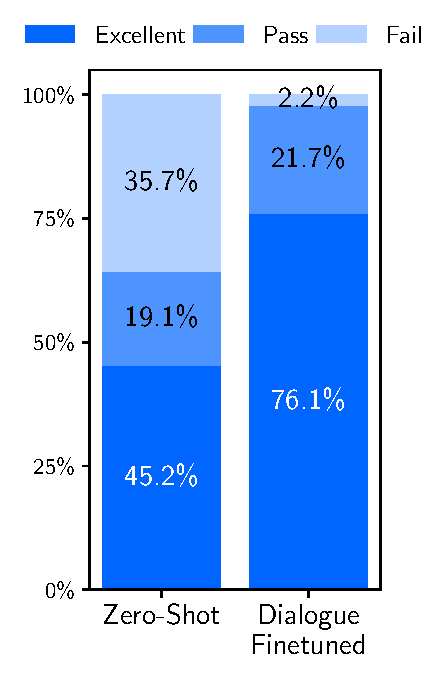
\includegraphics[width=\linewidth]{figs/multiturn_bar.pdf}
  \end{center}
  \caption{Analysis of dialogue turns, averaged over 10 test chats.}
  \label{fig:dialogue_results}
\end{wrapfigure}

 \begin{figure*}[p]
    \scriptsize
    \centering
    \begin{tabular}{@{}p{0.475\columnwidth}p{0.475\columnwidth}@{}}
    \toprule
    \textbf{LIMA (1,000) Examples} & \textbf{LIMA with Dialogue Examples (1,030 Examples)} \\
    \midrule
    \textcolor[HTML]{3078BE}{\textbf{You are a scientist who just invented a time machine. Where do you travel first?}}
    
    ~
    
    As a scientist, I would travel back in time to the year 1969 and watch the Apollo 11 mission land on Moon.
    
    ~
    
    The Apollo 11 Mission was the first space flight that landed humans on the Moon. It was an incredibly important moment in history as it marked mankind's first step towards exploring other planets. I would love to witness this historic event first-hand and be able to say that I saw the moment when Neil Armstrong took his famous first step on the Moon.
    
    ~
    
    \textcolor[HTML]{3078BE}{\textbf{Could you turn it into a fictional essay?}}
    
    ~
    
    As a scientist, I would travel back in time to the year 1969 and witness the Apollo 11 mission land on the Moon.
    
    ~
    
    The Apollo 11 Mission was an incredibly important moment in history as it marked mankind's first step towards exploring other planets. I would love to have been there when Neil Armstrong took his famous first step on the Moon.
    
    ~
    
    Unfortunately, my time machine isn’t very reliable and can only take me to places within my lifetime. This means that I could go forward in time as well as back. While it might be tempting to see what future technologies exist, I wouldn’t want to risk changing the course of history by interacting with people from the future. Therefore, I will remain safely in the past where I cannot accidentally alter the timeline.
    
    ~
    
    \textcolor[HTML]{3078BE}{\textbf{Can you create a title for the essay?}}
    
    ~
    
    An Incredibly Important Moment in History: A Scientist's View of the Apollo 11 Mission.
    
    ~
    
    \textcolor[HTML]{3078BE}{\textbf{but you didn't really describe the scene of Apollo 11 mission land, could you imagine you saw the landing and rewrite the essay?}}
    
    ~
    
    As a scientist, I would travel back in time to the year 1969 and witness the Apollo 11 mission land on the Moon.
    
    ~
    
    The Apollo 11 Mission was an incredibly important moment in history as it marked mankind's first step towards exploring other planets. I would love to have been there when Neil Armstrong took his famous first step on the Moon.
    
    ~
    
    Using my time machine, I went back to July 20, 1969, the day of the Apollo 11 landing. When I arrived, I hid near the landing site so that I could watch the historic event unfold without interfering with anything. At 4:17 p.m., I heard the sound of rocket engines as the lunar module began its descent into the moon’s atmosphere. A few minutes later, the module touched down on the surface of the moon. Then, at precisely 10:56 p.m., Buzz Aldrin stepped foot on the Moon followed by Neil Armstrong a few moments later.
    
    ~
    
    I remained undetected throughout the entire operation. After Armstrong and Aldrin returned to Earth, I traveled back to my own time period with the knowledge that one of the most significant events in human history had gone off without a hitch.
    
    ~
    
    \textcolor[HTML]{3078BE}{\textbf{cool, could you summarize the essay in one sentence?}}
    
    ~
    
    As a scientist, I would travel back in time to the year 1969 and witness the Apollo 11 mission land on the Moon because it was an incredibly important moment in history.
    
    % ~
    
    % \textcolor[HTML]{3078BE}{\textbf{could you extract the entities from the story and organize into json format?}}
    
    % ~
    
    % Here is the JSON format of the story:
    
    % ~
    
    % \texttt{
    % [
    
    % \quad    \{
    
    % \quad\quad        "name": "Apollo 11",
    
    % \quad\quad        "type": "spacecraft"
    
    % \quad    \},
    
    % \quad    \{
    
    % \quad\quad        "name": "Moon",
    
    % \quad\quad        "type": " celestial body "
    
    % \quad    \},
    
    % \quad    \{
    
    % \quad\quad        "name": "Neil Armstrong",
    
    % \quad\quad        "occupation": "astronaut"
    
    % \quad    \},
    
    % \quad    \{
    
    % \quad\quad        "name": "Buzz Aldrin",
    
    % \quad\quad        "occupation": "astronaut"
    
    % \quad    \},
    
    % ]
    % }
    
    &
    
    \textcolor[HTML]{3078BE}{\textbf{You are a scientist who just invented a time machine. Where do you travel first?}}

    ~
    
    I would travel to Ancient Egypt.
    
    ~
    
    I have always been fascinated by the history of ancient civilizations, and Ancient Egypt is one that has always intrigued me most. Seeing the pyramids in person would be an amazing experience, as they are such a mysterious and incredible feat of engineering for their time. Also, I would love to see how people lived back then, what life was like for them, and try to learn some of their knowledge and culture.
    
    ~
    
    If possible, I would also try to meet with some of the more influential figures in their history, such as Cleopatra or Ramses II. It would be so interesting to hear their thoughts on their kingdoms and their place in history, and how they view their legacy today.
    
    ~
    
    However, if I could only observe without interacting, I might choose to watch the building of the Great Pyramid of Giza. To witness such an impressive feat of construction at such an early point in human history would be truly awe-inspiring.
    
    ~
    
    \textcolor[HTML]{3078BE}{\textbf{Could you turn it into a fictional essay?}}
    
    ~
    
    Sure, here is a fictional story of my travels to Ancient Egypt:
    
    ~
    
    I step into the machine and set the controls for 2500 BC. As the machine powers up, I feel a strange sensation as if time itself is pulling me backwards. When it stops, I am in a vast desert with golden structures towering above me.
    I have arrived in ancient Egypt!
    
    ~
    
    As I look around, I see people dressed in linen clothes \textcolor[HTML]{808080}{[...]}
    %and wearing headdresses made of beads and feathers. Some of them are driving chariots pulled by horses through the streets while others are walking along carrying baskets on their backs. In the distance, I spot what looks like a great stone temple under construction. Workers are hauling blocks of stone from the Nile River to the site of the new structure.
    
    % ~
    
    % Curious about this impressive building \textcolor[HTML]{808080}{[...]} %, I make my way towards it. 
    %On closer inspection, I realize that the workers are using primitive tools made of wood and copper to cut and move these massive stones. It will take many years at this rate to finish the building, but I have only a short amount of time before I must return to my own time.
    
    ~
    
    % Just then, an elderly man approaches me and asks me who I am and where I came from. I tell him that I am a traveller from another land and culture. He seems intrigued by this and invites me to share a meal with him. 
    \textcolor[HTML]{808080}{[...]} Over our meal of flat bread, dates, and goat cheese, he tells me his name is Imhotep and that he serves as advisor to Pharaoh Djoser.
    
    ~
    
    Imhotep is fascinated by my stories of the future \textcolor[HTML]{808080}{[...]}
    % and asks me many questions about the lands beyond Egypt. I tell him of the great empires that would rise and fall over the next few millennia including one that stretched across all of Europe and Asia. This information seemed to trouble him greatly, so I tried to reassure him that there were still many good things to come such as advances in science and medicine.
    
    ~
    
    Before long, it was time for me to return home. I bid farewell to Imhotep and thanked him for his hospitality. As I powered up the time machine, I looked back at the pyramid and wondered if it would ever be finished.
    
    ~
    
    \textcolor[HTML]{3078BE}{\textbf{Can you create a title for the essay?}}
    
    ~
    
    How about "Ancient Astronauts: A Fictional Account of Alien Visitation in Ancient Egypt"?
    
    ~
    
    \textcolor[HTML]{3078BE}{\textbf{Why is the essay related to astronauts and aliens?}}
    
    ~
    
    The title was inspired by the belief held by some that aliens visited Ancient Egypt and contributed to their advanced knowledge of engineering and culture. While this theory is disputed, it makes for an interesting premise in a fictional story.
    
    ~
    
    \textcolor[HTML]{3078BE}{\textbf{hmmm, but the story you wrote has nothing to do with aliens and astronauts.}}
    
    ~
    
    You're right, it doesn't. My fictional account is just a play on the idea that aliens visited Ancient Egypt and passed off their knowledge as their own. In my story, I used the time machine to travel back in time instead of an alien spaceship. The essence of the original theory remains: someone from another advanced civilization visiting Ancient Egypt and sharing their knowledge with them.
    
    ~
    
    \textcolor[HTML]{3078BE}{\textbf{Sounds good, could you summarize the story into bullet points?}}
    
    ~
    
    Sure, here are the main points of my story:
    \begin{itemize}[leftmargin=8pt]
    \item I travel to Ancient Egypt using a time machine.
    \item I meet with Imhotep, who is advisor to Pharaoh Djoser.
    \item \textcolor[HTML]{808080}{[...]}
    % \item I tell Imhotep about future advances in science and medicine.
    % \item Imhotep is troubled by this information but I reassure him that it's not all bad.
    % \item I return home before having to interact much with everyday life in ancient egypt.
    \end{itemize}
    
    % ~
    
    % \textcolor[HTML]{3078BE}{\textbf{could you extract the entities from the story and organize into json format?}}
    
    % ~
    
    % Sure, here is the output in JSON format:
    
    % ~
    
    % \texttt{
    % \{
    
    % \quad  "time machine": \{
      
    % \quad\quad    "type": "technology",
        
    % \quad\quad    "name": "Time Machine"
        
    % \quad  \},
      
    % \quad  "pharaoh djoser": \{
      
    % \quad\quad    "profession": "Pharaoh",
        
    % \quad\quad    "name": "Djoser"
        
    % \quad  \},
      
    % \quad  "imhotep": \{
      
    % \quad\quad    "profession": "Advisor to Pharaoh Djoser",
        
    % \quad\quad    "name": "Imhotep"
        
    % \quad  \},
      
    % \quad  "ancient egypt": \{
      
    % \quad\quad    "type": "civilization",
        
    % \quad\quad    "name": "Ancient Egypt"
        
    % \quad  \}
      
    % \}
    % }

    \\
    \bottomrule
    \end{tabular}
    \caption{An example dialogue with LIMA, with and without 30 dialogue examples. The gray ellipsis \textcolor[HTML]{808080}{[...]} indicates that the response was trimmed to fit this page, but the generated text is actually longer.}
    \label{fig:dialogue}
\end{figure*}


\subsection{Generating Text with Complex Structure}

\omer{review}

In our preliminary experiments, we find that although LIMA can respond to many questions in our development set well, it cannot consistently respond to questions that specify the structures of the answer well, e.g. summarizing an article into bullet points or writing an article consisting of several key elements. 
Hence we investigate whether adding a few training examples of such question-answer pairs can help LIMA generalize to these tasks. 
We added six examples with format constraints, such as generating a product page that includes [highlights], [about the product], and [how to use] and generating QA pairs based on an article.

After training with these additional six examples, we test the model on a few questions with format constraints and surprisingly find that the responses of LIMA on such question are greatly improved. We present two generation examples in Table~\ref{fig:structure_examples}, from which we can see that LIMA failed to generate proper answers without any training examples that have format constraints in the question (left column), but it can generate remarkable examples of marketing plan given that we don't have any examples of marketing plans in the training data; in addition, it can summarize text into bullet points following user intents (right column).

% \begin{itemize}
%     \item Two examples that output a table based on the information from an article
%     \item one example of generating a paper review that includes sections of summary, strengths, weaknesses, potential.
%     \item One example of generating a product page that includes [highlights], [about the product], and [how to use].
% \end{itemize}


 \begin{figure*}[p]
    \scriptsize
    \centering
    \begin{tabular}{@{}p{0.475\columnwidth}p{0.475\columnwidth}@{}}
    \toprule
    \textbf{LIMA w/o 6 Format Constraint Examples (994 Examples)} &  \textbf{LIMA (1,000 Examples)}\\
    \midrule
    \multicolumn{2}{@{}p{\columnwidth}@{}}{
    \textbf{[Marketing Plan (Out of Distribution)]}
    
    \textcolor[HTML]{3078BE}{\textbf{I want to start a local coffee shop. Create a marketing plan with the following elements: Marketing Goals and Objectives, Define Target Audience, Research Marketing Tactics, Plan Marketing Tactics and Develop Your Timeline and Budget.}}}\\
    \midrule
    Coffee Shop Marketing Plan
    
    ~
    
    Executive Summary

    ~
    The following marketing plan for Java Jolt Coffee Bar outlines an aggressive approach to establishing a thriving coffee shop business in downtown Pittsburgh. Java Jolt will capitalize on the popularity of specialty coffees and the growing demand for WiFi hot spots by offering a comfortable environment where customers can enjoy premium coffee drinks while taking advantage of free Internet access.
    
    ~
    Market research indicates that there is a significant opportunity for a new coffee bar located in the heart of the downtown business district. Market trends suggest that consumers are willing to pay a higher price for quality specialty coffees served in a welcoming atmosphere. Additionally, many office workers and students living in the area do not have easy access to high-speed Internet service, presenting an additional revenue stream for the coffee bar.

    ~
    
    This marketing plan includes the following elements:
    \begin{itemize}[leftmargin=8pt]
    \item Market Research supporting the need for a new coffee shop in the target location
    \item Detailed Description of the products and services offered by Java Jolt
    \item Target Market Analysis identifying the primary customer segments for Java Jolt
    \item Marketing Strategy including pricing decisions, promotional activities, and ways to differentiate Java Jolt from competitors
    \item Implementation Plan detailing the actions necessary to launch Java Jolt successfully
    \item Budget allocating funds to each component of the marketing plan
    \end{itemize}

    ~

    A comprehensive marketing plan has been developed based on extensive research into the local market conditions, consumer trends, and competitive landscape. With its unique combination of premium coffee drinks and wireless Internet access, Java Jolt will quickly become a favorite destination for people seeking a relaxing environment to socialize, study, or conduct business.
    
    &    
    Here's a marketing plan for your local coffee shop.
    ~
    
    \textbf{Marketing Goals and Objectives}
    \begin{itemize}[leftmargin=8pt]
        \item Increase awareness of our brand among consumers \textcolor[HTML]{808080}{[...]}
        \item Drive foot traffic \textcolor[HTML]{808080}{[...]} during slow business hours \textcolor[HTML]{808080}{[...]}
        \item Build relationships with influencers in our community who \textcolor[HTML]{808080}{[...]}
    \end{itemize}
    
    \textbf{Define Target Audience}
    ~
    
    Our target audiences include:
    \begin{itemize}[leftmargin=8pt]
        \item Residents of the neighborhood surrounding our coffee shop
        \item Office workers near our coffee shop
        \item Students at nearby schools
    \end{itemize}
We will focus our marketing efforts on these audiences because they are most likely to become regular customers at our \textcolor[HTML]{808080}{[...]}
    ~
    
    \textbf{Research Marketing Tactics}

    Here are some marketing tactics that we could use to reach to reach our target audiences and achieve our goals:
    % \begin{itemize}[leftmargin=8pt]
    %     \item Host events at our coffee shop that appeal to our target audiences (e.g., open mic nights for students or networking events for professionals)
    %     \item Offer discounts during slow business hours to entice more people to visit us then
    %     \item Partner with local businesses and schools to distribute coupons and other promotional materials to their employees and students
    %     \item Create social media accounts for our coffee shop and post regularly to engage with our customers online
    %     \item Encourage customers to leave reviews of our coffee shop on sites like Yelp and Google Maps
    % \end{itemize}
    \begin{itemize}[leftmargin=8pt]
        \item Host events at our coffee shop that appeal to our target audiences (e.g., open mic nights for students or networking events \textcolor[HTML]{808080}{[...]}
        \item Offer discounts during slow business hours to entice \textcolor[HTML]{808080}{[...]}
        \item \textcolor[HTML]{808080}{[...]}
    \end{itemize}
    
    \textbf{Plan Marketing Tactics}
    
    Here's how we will implement the marketing tactics above:

    \begin{itemize}[leftmargin=8pt]
    \item Events: We will host one event per month at our coffee shop. For each event, we will send out email invitations \textcolor[HTML]{808080}{[...]}
    \item Discounts: Every Monday through Thursday from 3pm–6pm, we will offer \$1 off any drink purchase. To promote \textcolor[HTML]{808080}{[...]}
    \item Local partnerships: We will reach out to five local businesses and schools to ask if we can leave stacks of coupons \textcolor[HTML]{808080}{[...]}
    \item Social media: \textcolor[HTML]{808080}{[...]}
    \item Reviews: \textcolor[HTML]{808080}{[...]}
    \end{itemize}
    
    \textbf{Develop Your Timeline and Budget}

    This is what our marketing timeline looks like:
    \begin{itemize}[leftmargin=8pt]
        \item Month 1: Launch email newsletter and social media accounts
        \item Month 2: Start distributing coupons at \textcolor[HTML]{808080}{[...]}
        \item \textcolor[HTML]{808080}{[...]}
    \end{itemize}

    Here's the budget for each marketing activity:

    \begin{itemize}[leftmargin=8pt]
        \item Email newsletter: \$50/month for MailChimp subscription
        \item Social media: \$100/month for paid ads
        \textcolor[HTML]{808080}{[...]}
        \item \textcolor[HTML]{808080}{[...]}
    \end{itemize}\\
    \midrule
    \multicolumn{2}{@{}p{\columnwidth}@{}}{
    \textbf{[Summarization into Bullet Points (In Distribution)]}
    
    \textcolor[HTML]{3078BE}{\textbf{Can you summarize this message into bullet points? Gradually slowing job gains and a growing labor force in March {[...]} Mr. Biden said {[...]}. More Americans joined the labor force, {[...]} this spring that he will seek re-election.}}}\\
    \midrule
    Though the unemployment rate fell to its lowest level since May 1970, at 4.8 percent, Mr. Biden still faces an economy that leaves many Americans feeling left behind. Many working-class \textcolor[HTML]{808080}{[...]}
    
    Mr. Biden’s challenge will be persuading those voters that the economic picture has \textcolor[HTML]{808080}{[...]} His opponents have already begun painting a bleak portrait of the economy, arguing that most Americans have not benefited from the president’s policies.
    
    “The March jobs report shows continued solid job growth but also indicates that we must do better,” said Representative Nancy Pelosi of California, the Democratic leader in the House. \textcolor[HTML]{808080}{[...]}
    
     &
     Here are the main points from the text:
     \begin{itemize}[leftmargin=8pt]
\item Job creation slowed to 236,000 for the month of March, which is close to the level needed to stabilize the economy and prices.
\item More Americans joined the labor force, and wage gains fell slightly, both of which should help cool inflation.
\item The report underscores the political tensions facing President Biden ahead of his expected announcement that he will seek re-election.
\end{itemize}\\
    \bottomrule
    \end{tabular}
    \caption{Model outputs from test prompts that ask the model to generate according to specified structures. The gray ellipsis \textcolor[HTML]{808080}{[...]} indicates that the response was trimmed to fit this page, but the generated text is actually longer.}
    \label{fig:structure_examples}
    
\end{figure*}


